\documentclass{beamer}
\usepackage[spanish]{babel}
\usepackage[utf8]{inputenc}
\usepackage{graphicx}
\usepackage{xcolor}

\title{Moogle!: Proyecto de Programación I}
\author{Cristhian Delgado Garcia}
\date{}
\begin{document}
\definecolor{cyan_opaco}{RGB}{0,153,153} 
\definecolor{blue_opaco}{RGB}{0,0,153}
\newcommand{\class}[1]{\textcolor{cyan_opaco}{\texttt{#1}}}
\newcommand{\keyword}[1]{\textcolor{blue_opaco}{\texttt{#1}}}
\begin{frame}
\maketitle
\end{frame}

\begin{frame}{Introducción}
    \textbf{Moogle!} es un motor de búsqueda simple que usa el Modelo de Espacio Vectorial para encontrar los archivos de texto más relevantes para una consulta. A continuación se describen los conceptos matemáticos y la implementación en C\# de este proyecto.

\end{frame}
\begin{frame}{Desarrollo}
Se comienza seleccionando el conjunto de documentos con estensión \textit{.txt} en la carpeta \textit{Content} como se puede ver en la figura \ref{fig:carpetacontent}.
\begin{figure}
    \centering
    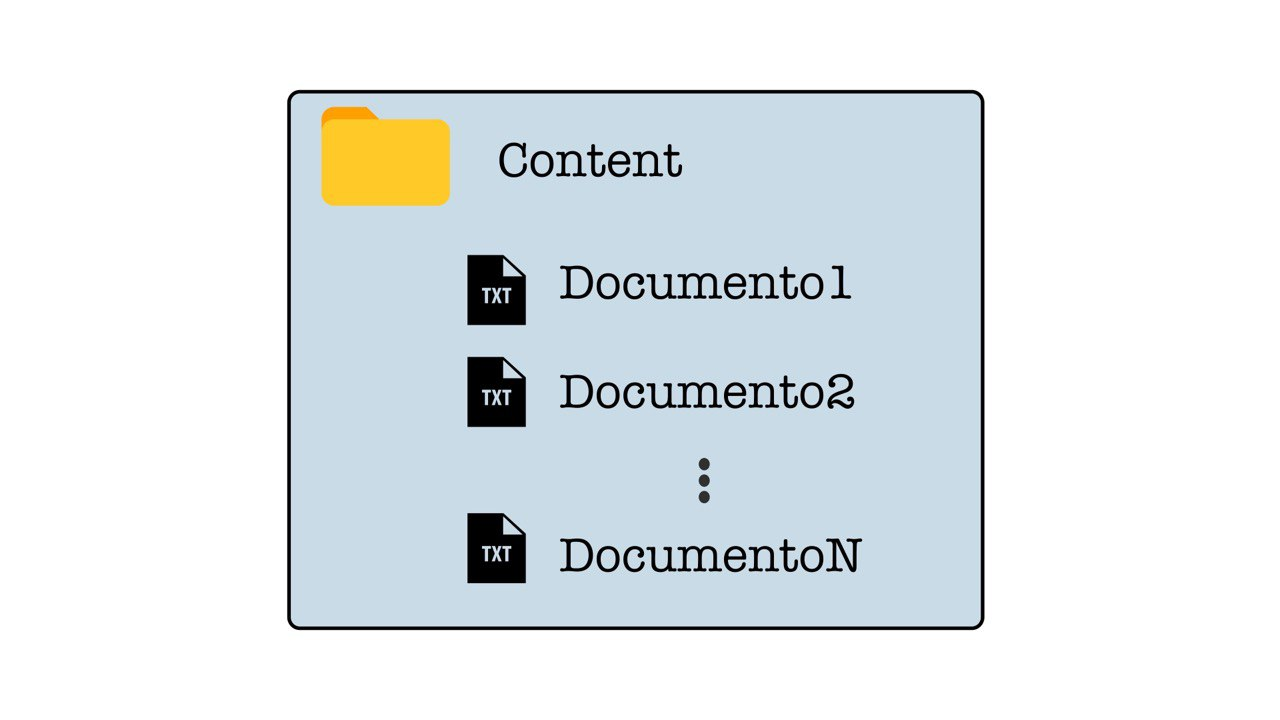
\includegraphics[width=0.5\linewidth]{content.jpg}
    \caption{Carpeta Content}
    \label{fig:carpetacontent}
\end{figure}
\end{frame}
\begin{frame}
Luego se crea un objeto \texttt{documents} de la clase \class{Documents} con la ruta de ese directorio . Este objeto tiene una propiedad fundamental: \texttt{TF\_IDF}.La propiedad es un \textit{array} bidimensional que representa la matriz con la medida \textit{tfidf}. Esta medida indica la relevancia de un término en un documento dentro de una colección, y se obtiene multiplicando la frecuencia del término (tf) por el inverso de la frecuencia del documento (idf), que es el logaritmo del cociente entre número de documentos y el número de documentos con el término.Aqui se muestra una posible representación de la matriz TF-IDF:
\begin{equation*}
\label{eq:matriztfidf}
\text{D} =
\begin{bmatrix}
\text{tfidf}(t_1, d_1) & \text{tfidf}(t_1, d_2) & \cdots & \text{tfidf}(t_1, d_n) \\
\text{tfidf}(t_2, d_1) & \text{tfidf}(t_2, d_2) & \cdots & \text{tfidf}(t_2 d_n) \\
\vdots & \vdots & \ddots & \vdots \\
\text{tfidf}(t_m, d_1) & \text{tfidf}(t_m, d_2) & \cdots & \text{tfidf}(t_m, d_n)
\end{bmatrix}
\end{equation*}
Como se aprecia el elemento en la posición (i,j) representa el tfidf del \textit{i}-ésimo término en el \textit{j}-ésimo documento.

\end{frame}
\begin{frame}
    Mientras se procesan los documentos tambien se renderiza la interfaz gráfica como se observa en la figura  \ref{fig:ui}, en donde el usuario podrá escribir su consulta.


    \begin{figure}
        \centering
        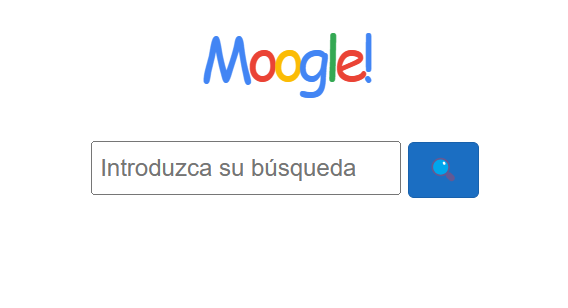
\includegraphics[width=0.75\linewidth]{ui.png}
        \caption{Interfaz Gráfica}
        \label{fig:ui}
    \end{figure}
\end{frame}
\begin{frame}
Al escribir el usuario su consulta se llama al método estático \texttt{Query} de la clase \class{Moogle}. Este método crea una instancia \texttt{userInp} de la clase \class{Query} con esa consulta que, igual que el objeto \texttt{documents} ,tiene una propiedad \texttt{TF\_IDF}. Esta propiedad almacena un \textit{array} de \keyword{double} con los tfidf de los términos del conjunto de documentos en esta consulta, se puede representar como un vector fila:

\begin{equation*}
q = \begin{bmatrix}
\text{tfidf}(t_1, q) & \text{tfidf}(t_2, q)& \cdots & \text{tfidf}(t_n, q)
\end{bmatrix}
\end{equation*}
Con el método estático \texttt{Cos()} de la clase \class{Vector} se calcula la \textbf{similitud coseno} entre el vector query y cada vector documento y se almacena en un array de \keyword{double} \texttt{scores}. La \textbf{similitud coseno} es una medida que dice que tan similares son el vector query y un vector documento, y se calcula como el cociente entre el producto punto de los vectores y el producto de sus respectivos módulos. Por supuesto mientras mayor sea este valor más \textbf{relevante} es ese documento para esa query. 

\end{frame}

\begin{frame}
Una posible interpretación geométrica para esta medida se puede observar en la figura \ref{fig:similitudcoseno}\footnote{De Svjo - Trabajo propio, CC BY-SA 3.0, https://commons.wikimedia.org/w/index.php?curid=16746151}:
\begin{figure}
    \centering
    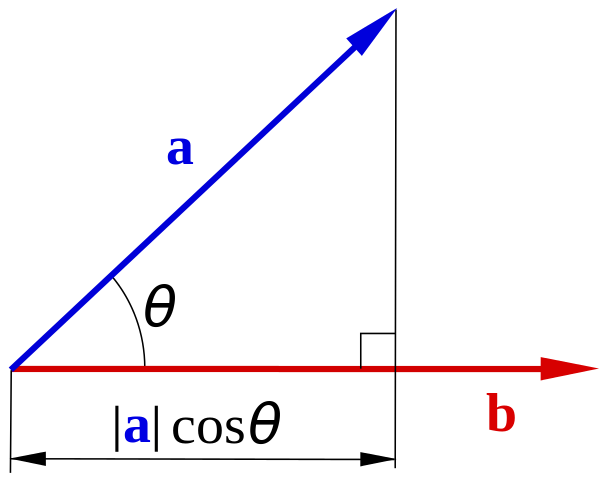
\includegraphics[width=0.5\linewidth]{605px-Scalar-product-dot-product.svg.png}
    \caption{Similitud coseno}
    \label{fig:similitudcoseno}
\end{figure}

\end{frame}
\begin{frame}
  Finalmente usando los métodos estáticos \texttt{Sort()} y \texttt{Reverse()} de la clase \textit{built-in} \class{Array}  se devuelve un objeto \class{SerachResult} con los documentos ordenados por su relevancia (si tienen alguna relevancia) para esa query y un fragmento de su texto que serán desplegados en la Interfaz Gráfica como se muestra en la figura \ref{fig:resultados} : 
  \begin{figure}
      \centering
      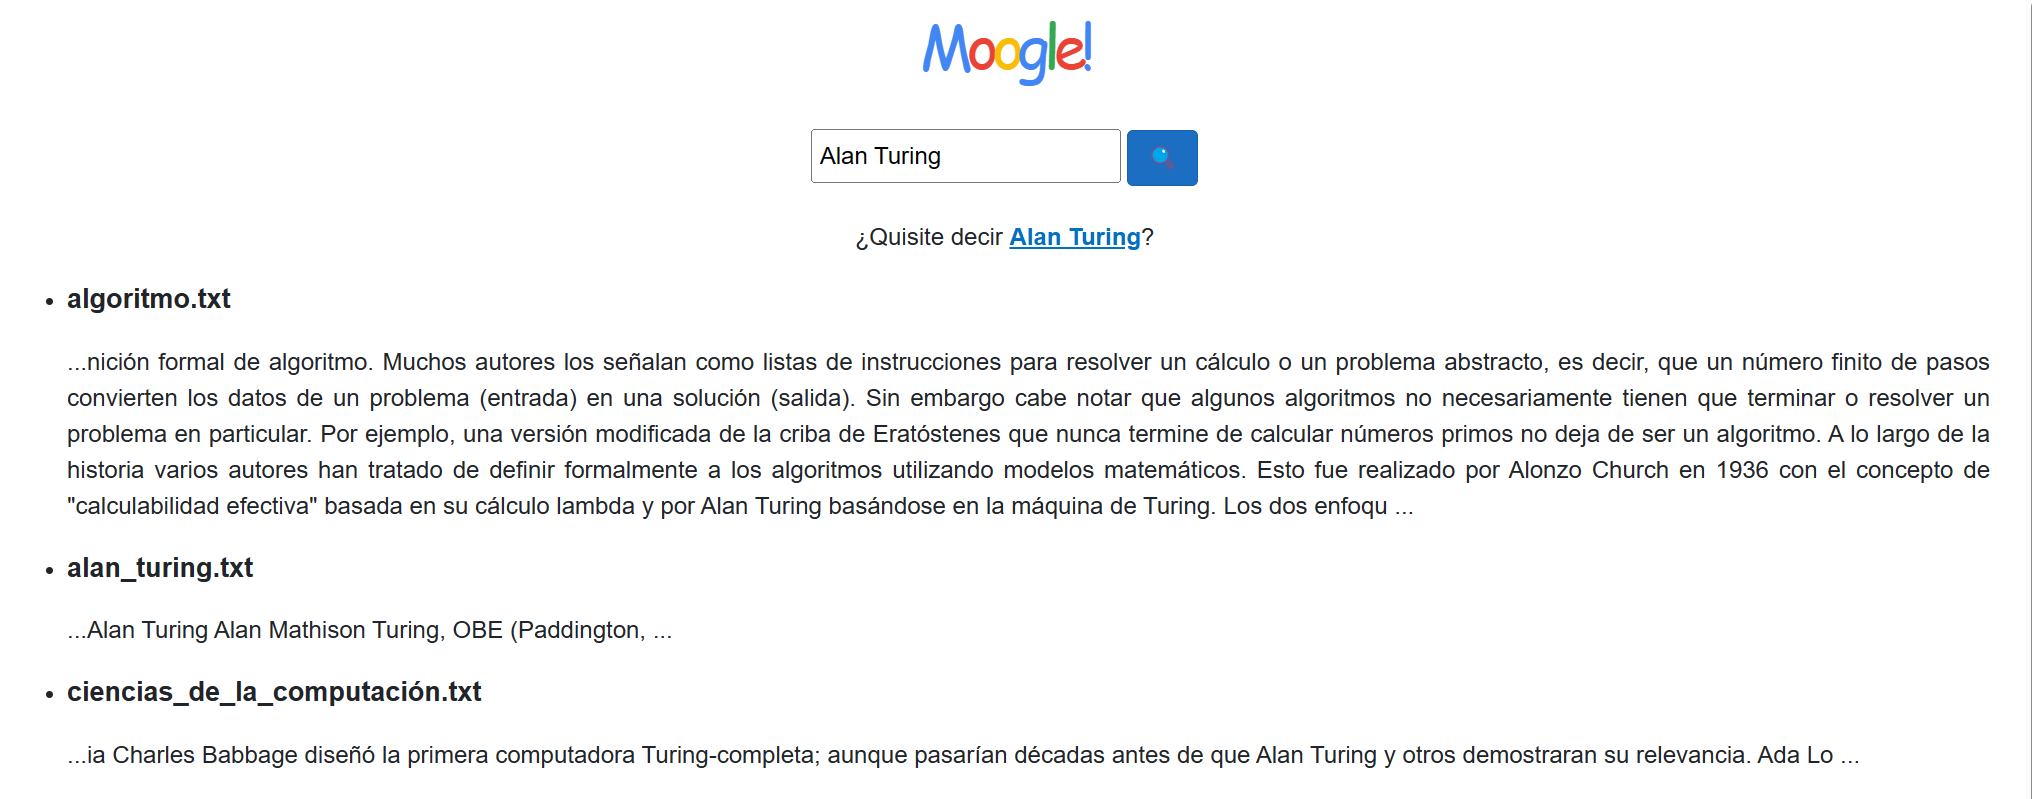
\includegraphics[width=1.\linewidth]{result.png}
      \caption{Resultados de una búsqueda}
      \label{fig:resultados}
  \end{figure}
\end{frame} 
\begin{frame}{Conclusiones}
Se concluye que \textbf{Moogle!} es un proyecto didáctico que ilustra los principios básicos de la recuperación de información y que ofrece una experiencia de búsqueda satisfactoria al usuario.
\end{frame}
\begin{frame}{Bibliografía }
\begin{itemize}
    \item Wikipedia 
    \item Chat Bing
    \item ChatGPT
\end{itemize}
\end{frame}
\end{document}